\tikzset{every picture/.style={line width=0.75pt}} %set default line width to 0.75pt

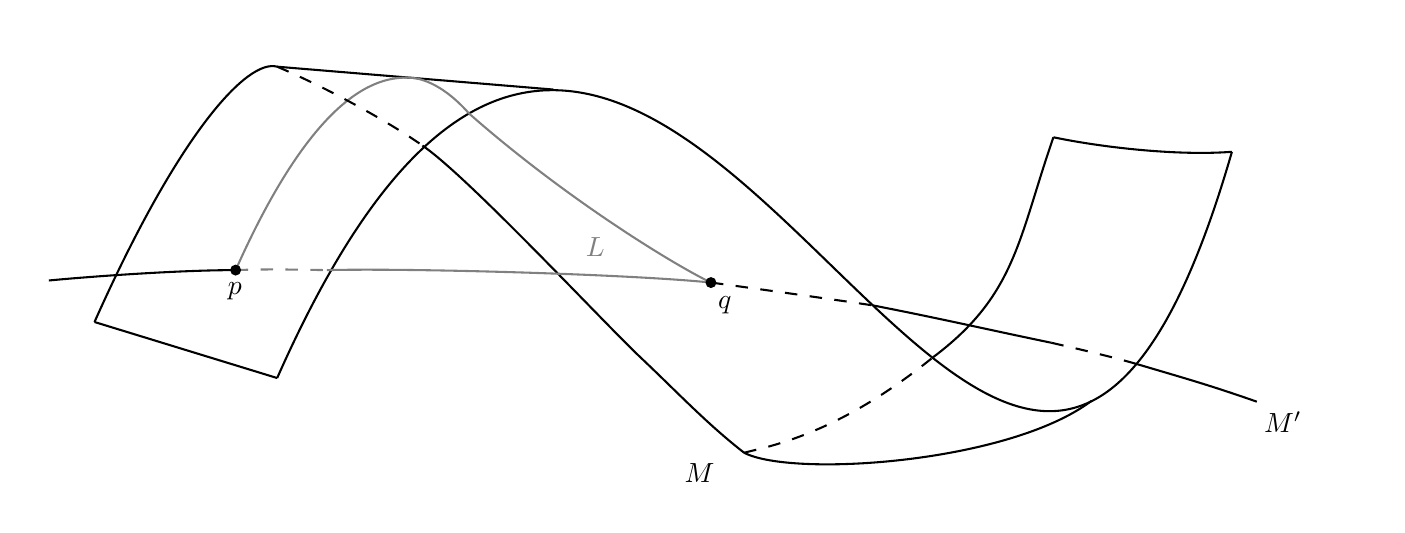
\begin{tikzpicture}[x=0.75pt,y=0.75pt,yscale=-1,xscale=1]
%uncomment if require: \path (0,724); %set diagram left start at 0, and has height of 724

%Curve Lines [id:da9620044273585225]
\draw    (140.2,413.8) .. controls (326.2,-6.2) and (486.2,699.8) .. (600.2,304.8) ;
%Curve Lines [id:da10895257227162702]
\draw    (52.2,386.8) .. controls (93.2,294.8) and (126.2,259.8) .. (140.2,263.8) ;
%Straight Lines [id:da8327014062778634]
\draw    (140.2,263.8) -- (273.2,274.8) ;
%Curve Lines [id:da4986053383299296]
\draw [color={rgb, 255:red, 128; green, 128; blue, 128 }  ,draw opacity=1 ]   (120.2,361.8) .. controls (161.2,269.8) and (192.7,267.9) .. (206.7,269.3) ;
%Straight Lines [id:da9571954478386947]
\draw    (52.2,386.8) -- (140.2,413.8) ;
%Curve Lines [id:da8062034220654326]
\draw    (30.2,366.8) .. controls (51.2,364.8) and (93.2,361.8) .. (120.2,361.8) ;
%Curve Lines [id:da40748546279172926]
\draw [color={rgb, 255:red, 128; green, 128; blue, 128 }  ,draw opacity=1 ] [dash pattern={on 4.5pt off 4.5pt}]  (120.2,361.8) .. controls (136.4,361.2) and (148.8,361.6) .. (164.2,361.8) ;
%Curve Lines [id:da8395773850437817]
\draw  [dash pattern={on 4.5pt off 4.5pt}]  (140.2,263.8) .. controls (166.2,274.8) and (196.2,291.8) .. (210.2,301.8) ;
%Curve Lines [id:da9403563547803104]
\draw    (210.2,301.8) .. controls (232.2,316.8) and (297.2,386.8) .. (315.2,403.8) .. controls (333.2,420.8) and (347.2,435.8) .. (365.2,449.8) ;
%Curve Lines [id:da21283109640207787]
\draw    (365.2,449.8) .. controls (388.2,461.8) and (492.4,454.9) .. (532.4,424.9) ;
%Curve Lines [id:da905844513019243]
\draw  [dash pattern={on 4.5pt off 4.5pt}]  (365.2,449.8) .. controls (376.2,446.8) and (409.2,441.8) .. (456.2,403.8) ;
%Curve Lines [id:da24023412254134335]
\draw    (456.2,403.8) .. controls (496.2,373.8) and (497.2,346.8) .. (514.2,297.8) ;
%Curve Lines [id:da617810943510469]
\draw    (514.2,297.8) .. controls (538.2,302.8) and (574.2,306.8) .. (600.2,304.8) ;
%Curve Lines [id:da05339788381467914]
\draw [color={rgb, 255:red, 128; green, 128; blue, 128 }  ,draw opacity=1 ]   (164.2,361.8) .. controls (205.2,360.8) and (310.2,363.8) .. (349.2,367.8) ;
%Curve Lines [id:da37032907704300666]
\draw  [dash pattern={on 4.5pt off 4.5pt}]  (349.2,367.8) .. controls (364.2,369.8) and (405.92,375.6) .. (427.2,378.8) ;
%Curve Lines [id:da5858810449257141]
\draw    (427.2,378.8) .. controls (458.2,384.8) and (484.2,390.8) .. (513.2,396.8) ;
%Curve Lines [id:da5792510662820718]
\draw  [dash pattern={on 4.5pt off 4.5pt}]  (513.2,396.8) .. controls (527.12,400) and (539.6,402.9) .. (553.52,406.8) ;
%Curve Lines [id:da04832578340355309]
\draw    (553.52,406.8) .. controls (575.3,413.3) and (588.3,416.8) .. (612.2,425.2) ;
%Curve Lines [id:da6743216618309311]
\draw [color={rgb, 255:red, 128; green, 128; blue, 128 }  ,draw opacity=1 ]   (206.7,269.3) .. controls (217.5,271.4) and (226.5,279.4) .. (232.7,286.4) ;
%Curve Lines [id:da6352281891905399]
\draw [color={rgb, 255:red, 128; green, 128; blue, 128 }  ,draw opacity=1 ]   (232.7,286.4) .. controls (279.3,327.4) and (330.8,358.9) .. (349.2,367.8) ;
%Shape: Circle [id:dp256915589824944]
\draw  [fill={rgb, 255:red, 0; green, 0; blue, 0 }  ,fill opacity=1 ] (118.1,361.8) .. controls (118.1,360.64) and (119.04,359.7) .. (120.2,359.7) .. controls (121.36,359.7) and (122.3,360.64) .. (122.3,361.8) .. controls (122.3,362.96) and (121.36,363.9) .. (120.2,363.9) .. controls (119.04,363.9) and (118.1,362.96) .. (118.1,361.8) -- cycle ;
%Shape: Circle [id:dp662684538575718]
\draw  [fill={rgb, 255:red, 0; green, 0; blue, 0 }  ,fill opacity=1 ] (347.1,367.8) .. controls (347.1,366.64) and (348.04,365.7) .. (349.2,365.7) .. controls (350.36,365.7) and (351.3,366.64) .. (351.3,367.8) .. controls (351.3,368.96) and (350.36,369.9) .. (349.2,369.9) .. controls (348.04,369.9) and (347.1,368.96) .. (347.1,367.8) -- cycle ;

% Text Node
\draw (114.9,366.4) node [anchor=north west][inner sep=0.75pt]    {$p$};
% Text Node
\draw (351.2,373.3) node [anchor=north west][inner sep=0.75pt]    {$q$};
% Text Node
\draw (287.4,344.4) node [anchor=north west][inner sep=0.75pt]  [color={rgb, 255:red, 128; green, 128; blue, 128 }  ,opacity=1 ]  {$L$};
% Text Node
\draw (335,453.4) node [anchor=north west][inner sep=0.75pt]    {$M$};
% Text Node
\draw (614.2,428.6) node [anchor=north west][inner sep=0.75pt]    {$M'$};

% 收紧图形边界框；不裁切也不改动任何曲线，只去除控制点造成的上下空白。
\pgfresetboundingbox
\path[use as bounding box] (20,245) rectangle (670,475);

\end{tikzpicture}
